
\section{Contrôle d’attitude du satellite \label{sec:3}} \label{partieIII}
\begin{obj}
L’objectif de cette partie est de mettre en place une loi de commande permettant d’asservir les
positions angulaires du satellite à des positions de référence. Dans les parties \autoref{sec:3:A}, \autoref{sec:3:B} et \autoref{sec:3:C},
il s’agira de déterminer le régulateur qui assure les performances de la chaîne d’asservissement.
Dans la partie \autoref{sec:3:D}, il s’agira de vérifier si la loi de commande déterminée permet de respecter
les contraintes imposées à l’actionneur : couple maximal et vitesse maximale qu’il peut réaliser.
%Dans le cas général, les lois de commande développées nécessitent une approche multivariable (trois
%axes), le cadre de ce sujet se restreint uniquement aux mouvements de tangage, soit à la rotation
%d’angle $\theta$  autour de l’axe $\vect{y}$. Les modèles utilisés ont été établis en adoptant $\psi  =\phi = 0$.
\end{obj}

\ifprof
\else

On rappelle que dans le mode de fonctionnement pointage fin (MNO) seuls les actionneurs par roues de réaction
et les magnétocoupleurs sont utilisés. Le cahier des charges partiel portant sur l’asservissement d’attitude est
détaillé dans le tableau de la \autoref{fig_09}. Ce cahier des charges doit être assuré même en cas d’un dépointage
initial qui sera modélisé comme condition initiale $\theta_0$ sur l’angle de tangage $\theta$. La consigne d’angle est notée $\theta_{\text{ref}}$ .

\begin{figure}[H]
\centering
\begin{tabular}{|p{.25\linewidth}|p{.35\linewidth}|p{.3\linewidth}|}
\hline
Chaîne d'asservissement & Ecart de pointage (en régimen permanent) & $| \Delta \theta | = | \theta_{\text{ref}}-\theta |\leq 0,04\degres$ \\
\cline{2-3}
& Pulsation de coupure $\omega_c à \SI{0}{dB}$ & $\SI{0,13}{rad.s^{-1}}$ \\ \cline{2-3}
& Marges de phase et de gain & $M\phi \geq 30\degres$ \\ \cline{2-3}
& & $MG \geq \SI{6}{dB}$ \\ \cline{2-3}
& Vitesse angulaire du satellite & $|\dot{\theta} | \geq  \SI{0,15}{\degres s^{-1}}$ \\ \hline
Actionneur à roue de réaction & Couple minimal & $|C|_{\text{max}} \leq \SI{0,005}{Nm}$ \\ \cline{2-3}
%& Couple minimal & $|C|_{\text{max}} \leq \SI{0,005}{Nm}$ \\ \hline
& Vitesse maximale & $|\Omega|_{\text{max}} \leq \SI{2800}{tr.min^{-1}}$ \\ \hline
Magnétocoupleurs & Couple maximal & $|C|_{\text{max}} \leq \SI{0,0005}{N.m}$ \\ \hline
Dépointage initial & Valeur maximale & $|\Theta|_{0} \leq \SI{20}{\degres}$ \\ 
\hline
\end{tabular}
%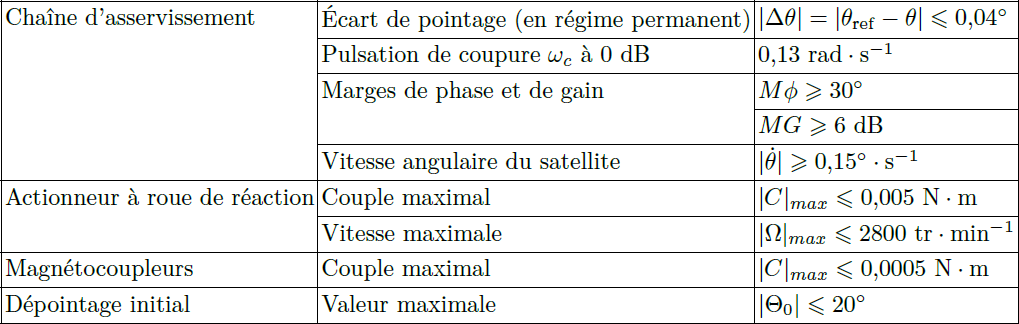
\includegraphics[width=\linewidth]{images/fig_09}
\caption{Cahier des charges pour la chaîne d’asservissement \label{fig_09}}

\end{figure}

L’architecture de contrôle d’attitude du satellite est représentée sur la \autoref{fig_10}. Dans le cas général, la loi de
commande utilise la mesure de la position angulaire du satellite et une estimation de sa vitesse. Dans le mode
de pointage fin, les actionneurs sont les roues de réaction qui fournissent un couple $C_{\text{roue}}$ conformément à un
couple de consigne $C_{\text{piloté}}$ demandé par la loi de commande. Le satellite est aussi soumis :
\begin{itemize}
\item à des couples perturbateurs sinusoïdaux de pulsations $\omega_0$ et $2\omega_{0}$ (avec $\omega_0 = \SI{0,001}{rad.s^{-1}}$) et d’amplitude,
dans le pire des cas, de $\SI{30e-6}{Nm}$;
\item à un couple constant d’amplitude $\SI{1e-6}{Nm}$.
\end{itemize}

\begin{figure}[H]
\centering
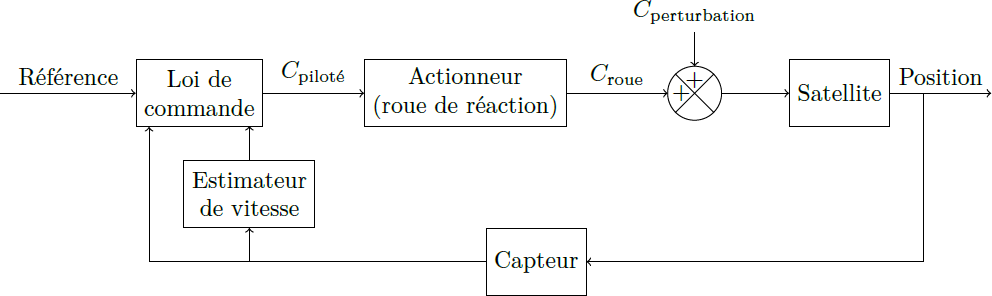
\includegraphics[width=.8\linewidth]{images/fig_10}
\caption{Architecture du système SCAO \label{fig_10}}
\end{figure}

Dans tous les modèles utilisés dans la suite, les angles sont exprimés en radians.

\fi

\subsection{\label{sec:3:A} Choix d’un modèle de commande et analyses préliminaires}

\ifprof
\else


La  \autoref{fig_11} montre la chaîne de régulation (monoaxe) où $H(p)$, $A(p)$ et $B(p)$ sont les fonctions de transfert modélisant respectivement le satellite, la roue de réaction et le capteur. On suppose dans un premier temps que l’actionneur et le capteur ont tous deux un gain statique unitaire mais sont affectés d’un retard pur : \SI{100}{ms} pour la roue de réaction et \SI{700}{ms} pour les capteurs stellaires. 
%La fonction de transfert du satellite est obtenue à partir des relations obtenues à la question \ref{q_8} ; et au regard de la bande passante souhaitée, on admettra qu’elle peut être approchée par la fonction $H(p)$ donnée ci-dessous. 
Ainsi, les fonctions de transfert correspondant aux différents éléments de la chaîne d’asservissement sont :
$$
H(p)=\dfrac{0,028}{p^2} 
\quad \quad 
A(p)=A_r (p) e^{-0,1p}\simeq \dfrac{1}{1+\dfrac{1}{0,87}p}e^{-0,1 p} 
\quad \quad 
B(p)=e^{-0,7p}
$$


Enfin, le correcteur représenté par la fonction de transfert $C(p) = R(p) F(p)$ est le produit de deux termes :
\begin{itemize}
\item $R(p)$ correspond à un régulateur de type PID (proportionnel, intégral, dérivé), qu’il s’agira de déterminer
dans la suite ;
\item $F(p)$ est la fonction de transfert d’un filtre de type passe-bas. Il a comme objectif de réduire le gain du système
en haute fréquence afin de ne pas exciter les modes oscillants (l’analyse de l’influence de ces modes est hors
du cadre de cette étude). Cette fonction de transfert sera approchée par la forme suivante 
$F(p) = \dfrac{1}{1 + 1,5p}$ (en pratique, ces filtres sont d’ordre 2).
\end{itemize}
\fi

\ifprof
\else

\begin{figure}[H]
\centering
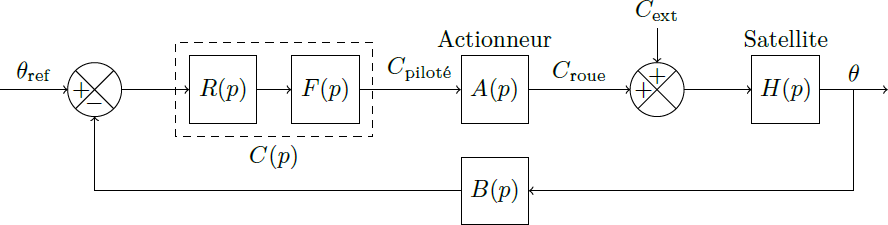
\includegraphics[width=.8\linewidth]{images/fig_11}
\caption{Schéma-bloc de la boucle d’asservissement d’attitude \label{fig_11}}
\end{figure}

\fi


\question{\textit{Exprimer $\theta$ en fonction de $\indice{\theta}{ref}$, $\indice{C}{ext}$ et des différentes fonctions de transfert.}}

\question{\textit{La figure du document réponse donne le diagramme de Bode de la fonction $A_r(p)H(p)F(p)$. Tracer directement sur cette figure les diagrammes asymptotiques associés à cette fonction (document réponse à rendre avec la copie). Vous justifirez le tracé en utilisant un tableau de variation. \label{q_15}}}
\ifprof
\begin{corrige}
Les pentes des asympotes sont données par le tableau suivant. 
\begin{figure}[H]
\centering
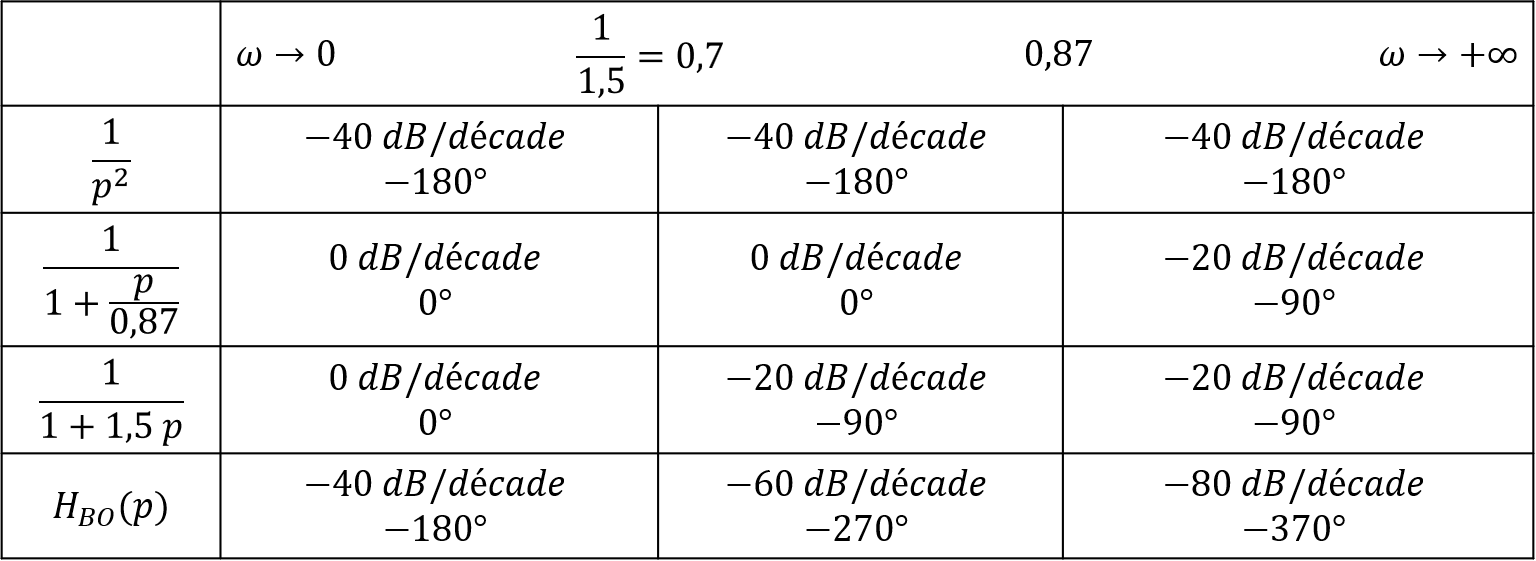
\includegraphics[width=.8\linewidth]{images/cor_q15}

%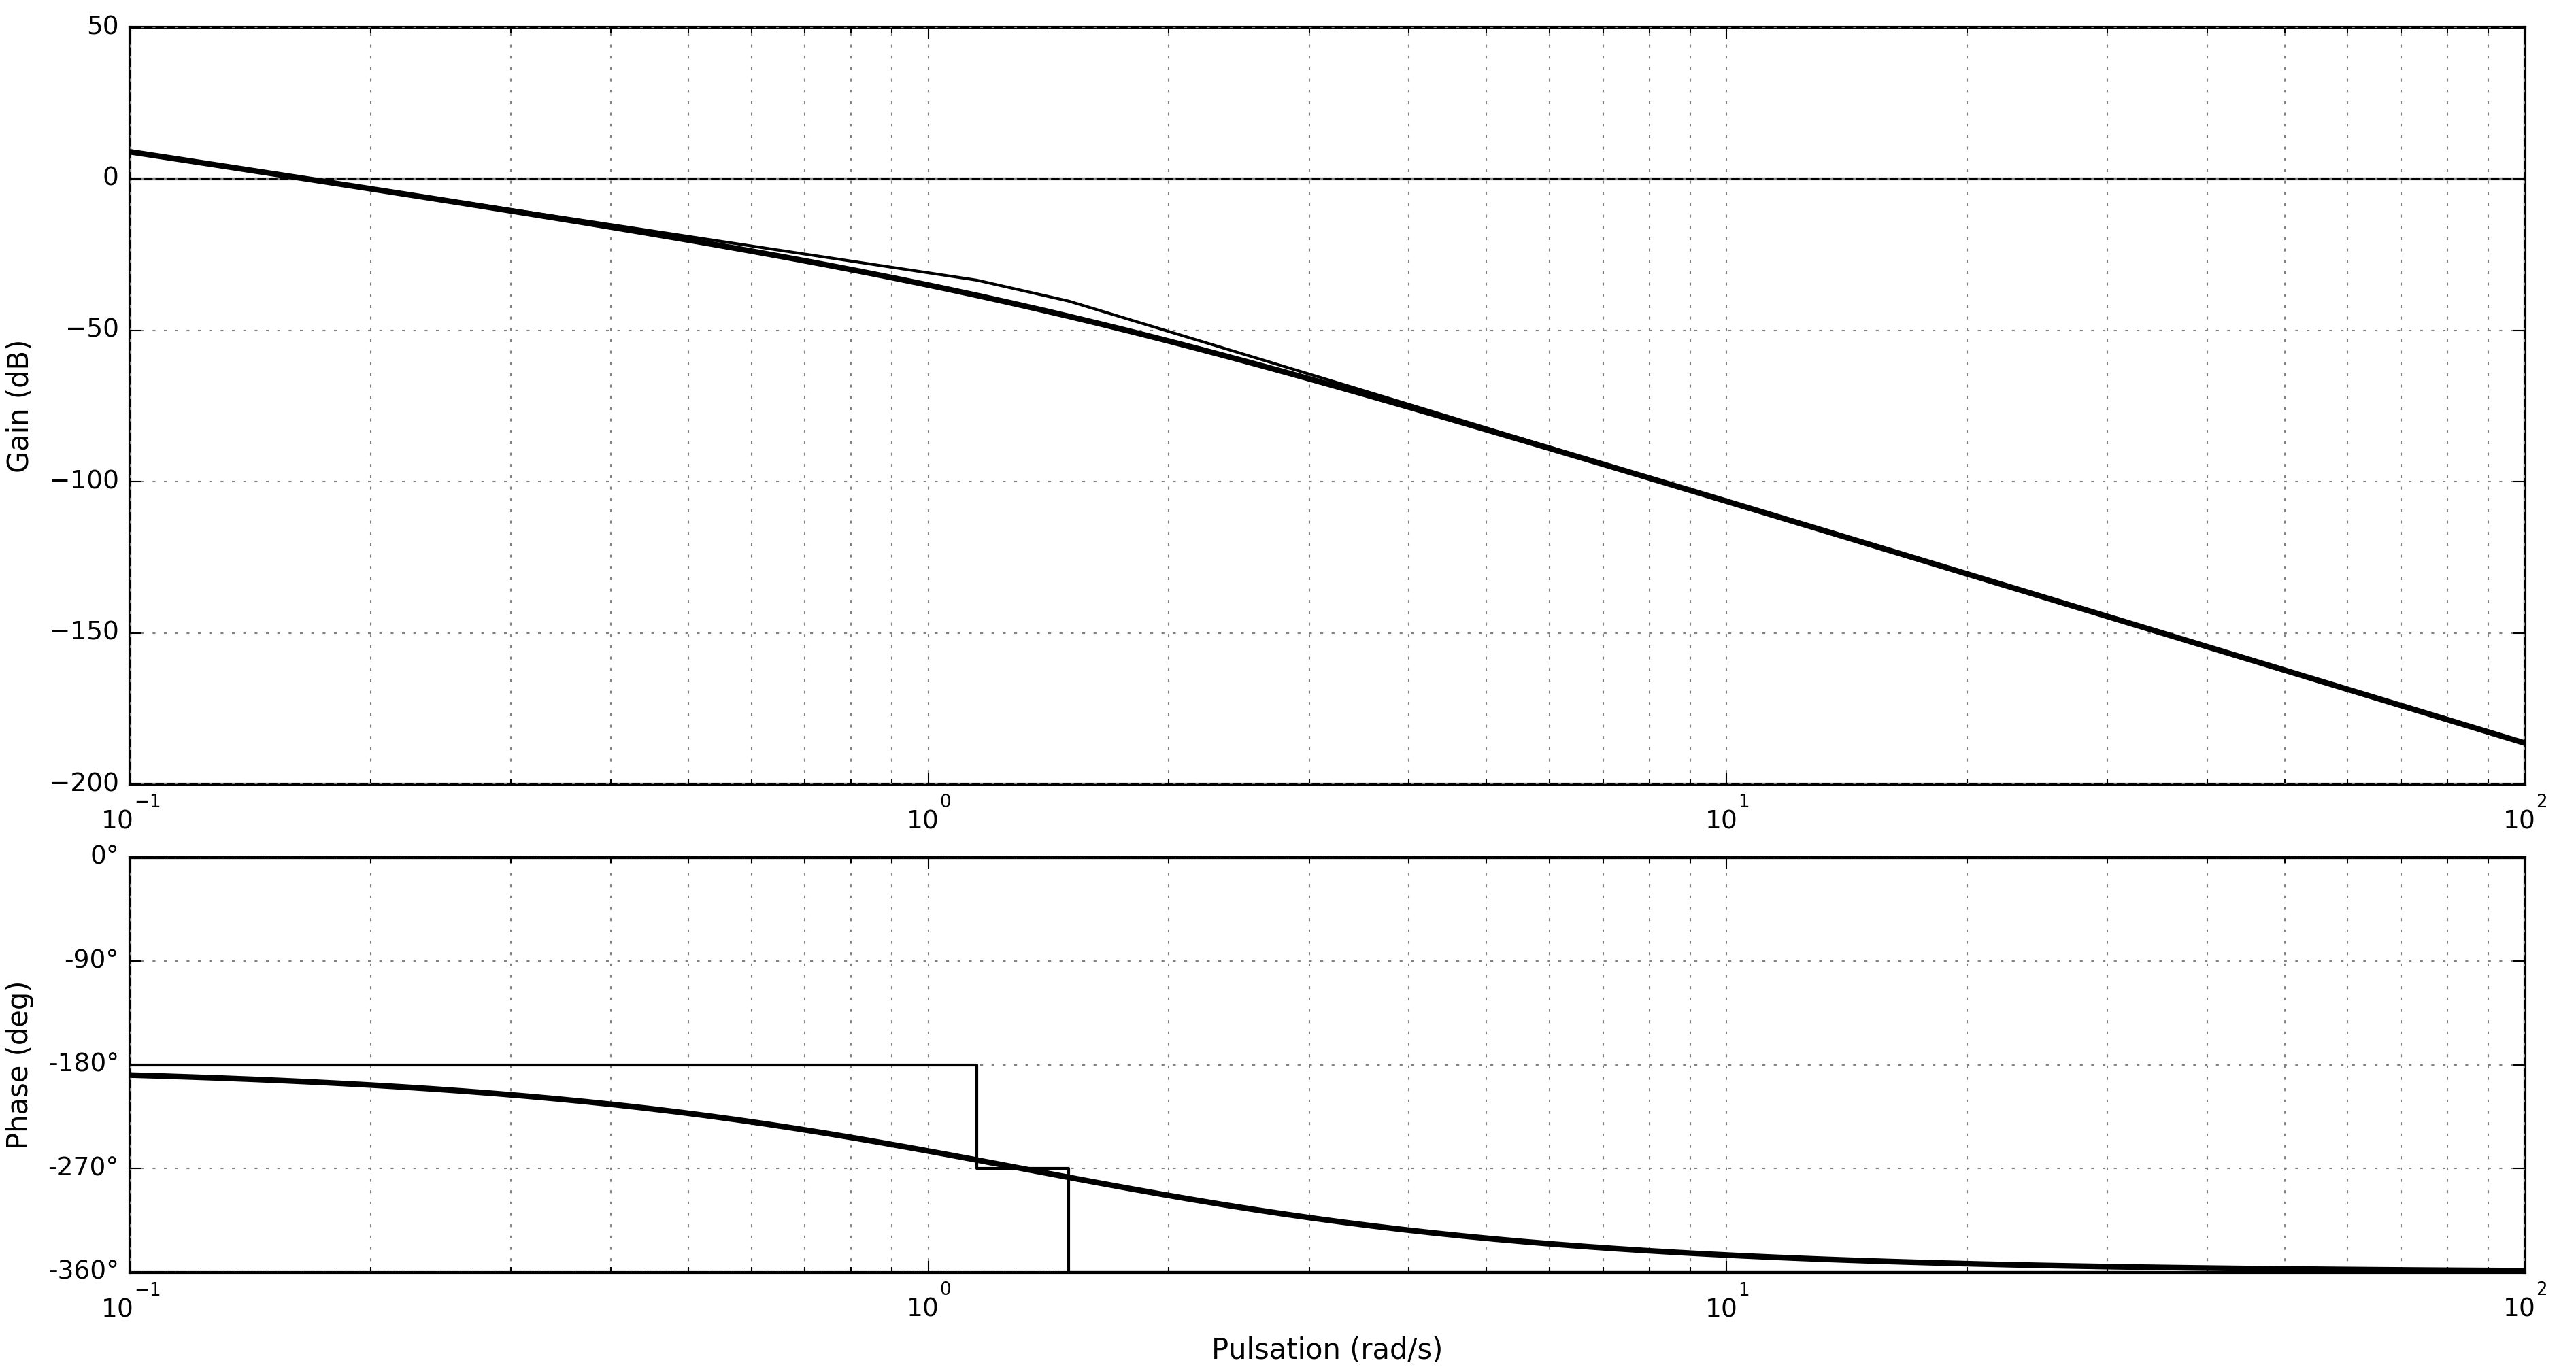
\includegraphics[width=.8\linewidth]{images/cor_q15_bode}
%\caption{Architecture du système SCAO \label{fig_10}}
\end{figure}


\end{corrige}


\begin{corrige}
\begin{figure}[H]
\centering

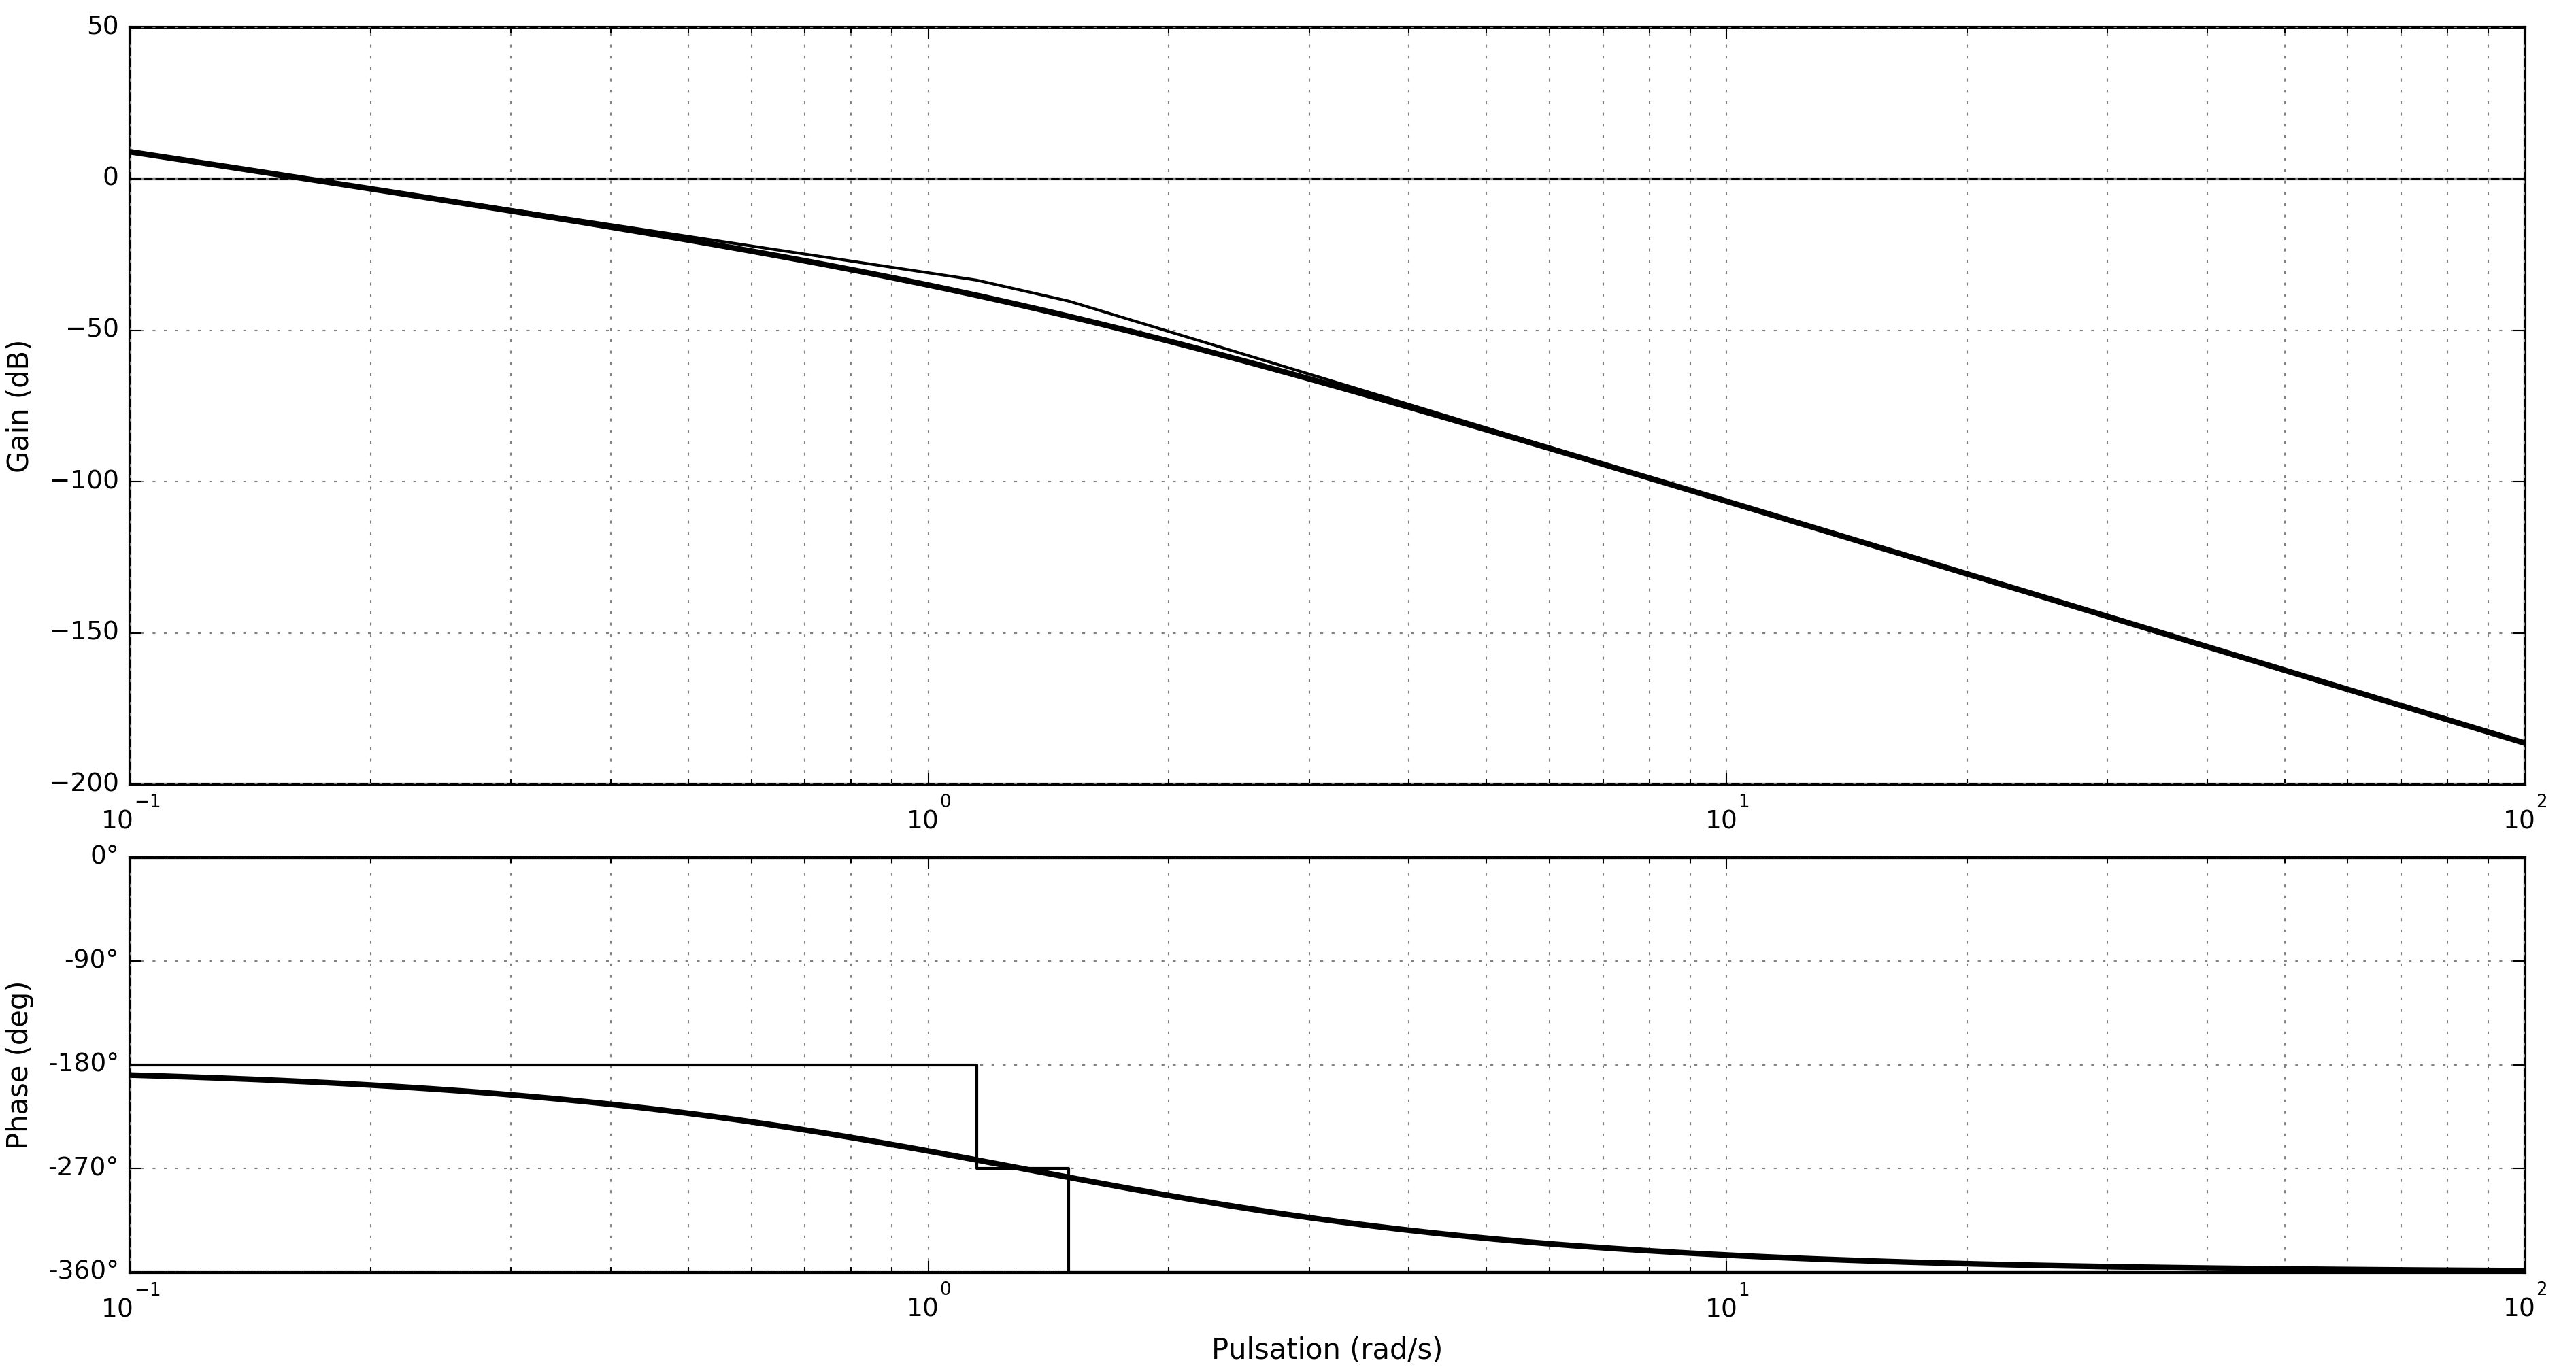
\includegraphics[width=.8\linewidth]{images/cor_q15_bode}
%\caption{Architecture du système SCAO \label{fig_10}}
\end{figure}

De plus, en basse fréquence, lorsque 
$\omega << \SI{0,1}{rad.s^{-1}}$, 
$H_{\text{BO}}(p)\simeq \dfrac{0,028}{p^2}$. 
On a donc  en $\omega = \SI{0,01}{rad.s^{-1}}$, $G_{\text{dB}}(0,01)\simeq 20\log \left(\dfrac{0,028}{0,01^2}\right)\simeq \SI{50}{dB}$.


\end{corrige}
\else
\fi

\question{\textit{En prenant $R(p) = 1$, préciser la fonction de transfert en boucle ouverte et tracer les diagrammes de
Bode réels (5 ou 6 points judicieusement choisis suffisent pour ces tracés) sur la figure B. Au regard des tracés
effectués, justifier que des corrections proportionnelle ou proportionnelle-intégrale ne permettent pas d’assurer
le cahier des charges escompté.\label{q_16}}}
\ifprof
\begin{corrige}
On a $\text{FTBO}(p)=F(p)A(p)H(p)B(p)=\dfrac{1}{1 + 1,5p} \dfrac{1}{1+\dfrac{1}{0,87}p}e^{-0,1 p}  \dfrac{0,028}{p^2} e^{-0,7p}$. Il s'agit donc d'ajouter le retard $e^{-0,8 p}$.

Le gain du retard est unitaire. Il ne change donc pas le diagramme de gain.
Le déphase ajouté par le retard est de $-0,8\omega $. 
On << descend >> donc la phase des valeurs suivantes. 

\begin{figure}[H]
\centering
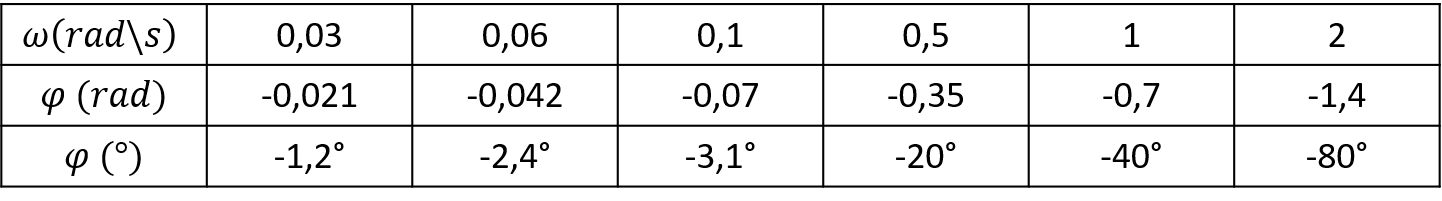
\includegraphics[width=.8\linewidth]{images/cor_q16}
%\caption{Architecture du système SCAO \label{fig_10}}
\end{figure}


\end{corrige}

\begin{corrige}




\begin{figure}[H]
\centering
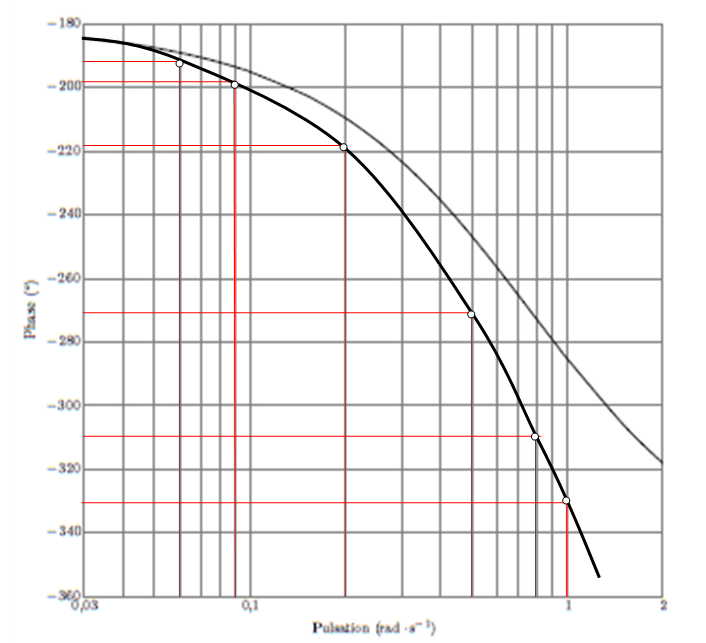
\includegraphics[width=.6\linewidth]{images/cor_q16_bis}
%\caption{Architecture du système SCAO \label{fig_10}}
\end{figure}


Cahier des charges :
\begin{itemize}
\item écart de pointage : avec un double intégrateur, le système est précis pour une entrée échelon -- exigence respectée;
\item pulsation de coupure à $\SI{0}{dB}= \SI{0,13}{rad.s^{-1}}$ -- exigence respectée (et réglable avec des correcteurs P et PI);
\item marge de phase : avec un système de classe 2, la phase est forcément inférieure à $-\SI{180}{\degres}$ -- exigence qui ne pourra pas être respectée avec un P ou un PI;
\item marge de gain : si la marge de phase n'est pas respectée, on ne pourra pas stabiliser le système...
\end{itemize}

\end{corrige}
\else
\fi


\question{\label{q_17}\textit{En déduire les conditions sur le module et l’argument de $R(j\omega)$ pour assurer la pulsation de coupure et
la marge de phase demandées par le cahier des charges associé au modèle nominal.}}
\ifprof
\begin{corrige}
En utilisant la BO non corrigée, on mesure :
\begin{itemize}
\item $\omega_{\SI{0}{dB}} = \SI{0,16}{rad.s^{-1}}$;
\item $M_{\varphi}=-\SI{25}{\degres}$
\end{itemize}
Le cahier des charges demande 
\begin{itemize}
\item $\omega_{\SI{0}{dB}} = \SI{0,13}{rad.s^{-1}}$;
\item $M_{\varphi}\geq \SI{30}{\degres}$, il faut donc que $\arg\left(R(j\omega_{\SI{0}{dB}}) \right)=45\degres$.
\item $M_{G}\geq \SI{6}{dB}$.
\item Dans ces conditions, il faudrait déterminer la pulsation pour laquelle la phase vaut $-180\degres$ puis ajuster le gain.
\end{itemize}
\end{corrige}
\else
\fi







\subsection{\label{sec:3:B} Analyse des contraintes sur la loi de commande}

\ifprof
\else

L’objet de cette partie est de déterminer les contraintes que doit vérifier le régulateur en vue d’assurer les
exigences de précision lorsque le procédé est soumis aux couples perturbateurs sinusoïdaux, c’est-à-dire de la
forme 
$c_{\text{ext}} = C_{00}\sin(\omega_0 t)$ et 
$c_{\text{ext}} = C_{01} \sin(2\omega_0t)$, 
dont les caractéristiques, amplitude et pulsation, sont données
précédemment : $C_{00} = C_{01} = \SI{30e-6}{N.m}$  et $\omega_0 = \SI{0,001}{rad.s^{-1}}$.
\fi


\question{\label{q_18}\textit{En prenant une consigne $\theta_{\text{ref}} = 0$, déterminer la fonction de transfert $T(p) = \dfrac{\theta(p)}{C_{\text{ext}}(p)}$ entre les couples perturbateurs $C_{\text{ext}}(p)$ et la position $\theta(p)$ et l’exprimer à partir des fonctions de transfert de la \autoref{fig_11}.}}
\ifprof
\begin{corrige}
On a $T(p)=\dfrac{H(p)}{1+H(p)B(p)A(p)C(p)}$ ou encore $T(p)=\dfrac{H(p)}{1+H(p)B(p)A(p)F(p)R(p)}$
\end{corrige}
\else
\fi

\question{\label{q_19}\textit{En utilisant les approximations fréquentielles 
$||T_{\text{bo}}(j\omega)||>>1$ et
$||T_{\text{bo}}(j\omega)||<<1$
où $T_{\text{bo}}(p)$ est la fonction
de transfert en boucle ouverte, montrer que dans l’intervalle des pulsations des couples perturbateurs, 
on peut écrire : 
$||T(j\omega)||\simeq \dfrac{1}{|| R\left(j\omega\right) F\left(j\omega\right) A\left(j\omega\right) B\left(j\omega\right)|| }$. 
 Justifier que cette relation peut encore être simplifiée selon la formulation :
 $||T(j\omega)||\simeq \dfrac{1}{|| R\left(j\omega\right)||}$.}}

\ifprof
\begin{corrige}
Pour des pulsations comprises entre $\SI{0,001}{rad.s^{-1}}$ et $\SI{0,002}{rad.s^{-1}}$, la FTBO tend vers $H(p)R(p)$.
Le gain est de la FTBO y est supérieur à \SI{40}{dB}. On peut donc considérer que 
$||T(j\omega)||\simeq \dfrac{||H\left(j\omega\right)||}{|| H\left(j\omega\right) R\left(j\omega\right) F\left(j\omega\right) A\left(j\omega\right) B\left(j\omega\right)|| } = \dfrac{1}{|| R\left(j\omega\right) F\left(j\omega\right) A\left(j\omega\right) B\left(j\omega\right)|| }$.

Or, $||F\left(j\omega\right) A\left(j\omega\right) B\left(j\omega\right)|| \simeq 0$ entre  entre $\SI{0,001}{rad.s^{-1}}$ et $\SI{0,002}{rad.s^{-1}}$; donc $||T(j\omega)||\simeq \dfrac{1}{|| R\left(j\omega\right)||}$.

\end{corrige}
\else
\fi

\question{\label{q_20}\textit{Donner l’expression de l’amplitude de  l'évolution temporelle de $\theta(t)$, en fonction de 
de $|| R\left(j \omega\right)||$,  en réponse
au couple perturbateur sinusoïdal de pulsation $\omega_0$. En déduire la condition que doit vérifier $|| R\left(j \omega\right)||$ en vue de
satisfaire la précision d’écart de pointage, pour une consigne $\theta_{\text{ref}} = 0$, lorsque le satellite est soumis à ce couple
perturbateur. Reprendre cette analyse dans le cas du couple 
perturbateur de pulsation $2\omega_0$.}}
\ifprof
\begin{corrige}
La perturbation étant sinusoïdale de la forme 
$c_{\text{ext}} = C_{00}\sin(\omega_0 t)$ on a 
$\theta(t)=K C_{00}\sin(\omega_0 t + \varphi)$ avec 
$K = \dfrac{1}{|| R\left(j\omega_0\right)||} $ et 
$\varphi = \arg\left( T(j\omega_0) \right)$.

D'après le cahier des charges, l'écart de pointage doit rester inférieur à $\SI{0,04}{\degres} = \SI{7e-4}{rad}$.
De plus, $C_{00}=C_{01}$; donc $K C_{00} <  \SI{7e-4}{rad} \Rightarrow K < \dfrac{7\times 10^{-4}}{30\times 10^{-6}} = \SI{23}{rad.N^{-1}m^{-1}}$ et $|| R\left(j\omega_0\right)|| > \SI{0,043}{Nmrad^{-1}}$.

\end{corrige}

\else
\fi

\subsection{\label{sec:3:C} Synthèse du régulateur}

Pour la synthèse du régulateur $C(p)$, on recherche une solution de la forme : $R(p)=K \dfrac{\left(1+\tau p\right)^2}{p}$.

\question{\label{q_21}\textit{Déterminer la valeur de $\tau$  permettant d’obtenir la marge de phase $M_{\varphi} = 30\degres$
 exigée par le cahier des charges.}}
\ifprof
\begin{corrige}
On a $\arg{R(p)} = \arg{K}+ \arg{\left(1+\tau p\right)^2} - \arg{p}$
$ =-\dfrac{\pi}{2}  +2 \arctan\left(\tau \omega \right)$.

D'après la question \ref{q_17}, l'apport de phase ajouté doit être de \SI{55}{\degres} pour une pulsation de $ \SI{0,13}{rad.s^{-1}}$; donc $55=-90  +2 \arctan\left(\tau 0,13 \right) $ et $\tau = \tan \left(\dfrac{55+90}{2}\right) \dfrac{1}{0,13} = \SI{24,4}{s}$.
\end{corrige}
\else
\fi 



\question{\label{q_22}\textit{En conservant la valeur de $\tau$ déterminée précédemment, calculer la valeur du gain $K$ qui assure la pulsation de coupure imposée par le cahier des charges.}}
\ifprof
\begin{corrige}
On a $||T_{\text{bo}}(j\omega)||=||H(j\omega)B(j\omega)A(j\omega)F(j\omega)R(j\omega)||$
$=0,028 \dfrac{1}{\omega^2}\dfrac{1}{\sqrt{1+\dfrac{\omega^2}{0,87^2}}}\dfrac{1}{\sqrt{1+\omega^2 1,5^2}} K \dfrac{1+\tau^2\omega^2}{\omega}$.

Pour $\omega = \omega_{\SI{0}{dB}}=\SI{0,13}{rad.s^{-1}}$ et $\tau=\SI{24,4}{s}$; 
$||T_{\text{bo}}(j\omega_{\SI{0}{dB}})|| = 136,8 K$. On souhaite que le gain dB soit nul (et donc le module unitaire); donc $K= \dfrac{1}{136,8} = 0,0073$.
\end{corrige}
\else
\fi

\question{\label{q_23}\textit{Vérifier si le régulateur déterminé permet d’assurer les conditions nécessaires à satisfaire les performances,
en termes d’écart de l’angle de pointage, lorsque le satellite est soumis aux variations sinusoïdales du couple
perturbateur.}}
\ifprof
\begin{corrige}

Si on considère qu'en basses fréquences,  $||T(j\omega)||\simeq \dfrac{1}{|| R\left(j\omega\right)||}$.


$|| R\left(j\omega\right)|| = \left|\left| 0,073  \dfrac{\left(1+24,4 j \omega\right)^2}{j\omega}\right|\right|$
$=0,073  \dfrac{ \left|\left| 1+24,4 j \omega \right|\right| ^2}{ \left|\left| j\omega\right|\right|}$
$=0,073  \dfrac{ 1+24,4^2  \omega^2 }{ \omega}$

Pour une perturbation sinusoïdale, l'amplitude de $\theta$ est donnée par $||T(j\omega)|| C_{00}$.  D'où :
\begin{itemize}
\item pour $\omega = \SI{0,001}{rad.s^{-1}}$, $||T(j\omega)|| C_{00} = 0,14 \times 30 \times 10^{-6} = \SI{5.8e-6}{rad} = 0,0003\degres\leq 0,04\degres$;
\item pour $\omega = \SI{0,002}{rad.s^{-1}}$, $||T(j\omega)|| C_{00} = 0,27 \times 30 \times 10^{-6} = \SI{2,2e-5}{rad} = 0,0012\degres\leq 0,04\degres$.
\end{itemize}
%on a, 
% dans le pire des cas, $||T(0,002 j)|| = \dfrac{1}{\left|\left| 0,073  \dfrac{\left(1+24,4 j \omega\right)^2}{j\omega}\right|\right|} = \left(0,0073 \dfrac{1+24,4^2\times 0,002^2}{0,002}\right)^{-1/2} \simeq (3,6)^{-1} =0,28$. On a $0,28\times 30\times 10^{-6}=4,77\times 10^{-4} \degres<0,04\degres$.
%  ***(AN à vérifier))
%  
\end{corrige}
\else
\fi

\subsection{\label{sec:3:D} Validation de la loi de commande}
\ifprof
\else
\begin{obj}
L’objectif de cette partie est de vérifier que les commandes issues du régulateur précédent ne
génèrent pas de contraintes excessives sur l’actionneur, en particulier que la vitesse maximale
et le couple maximal restent dans les « limites » de l’actionneur réalisé par la roue de réaction.
Cette vérification se fera d’une part vis-à-vis d’un dépointage initial et d’autre part vis-à-vis des
différents couples perturbateurs. Enfin, une modification de la loi de commande sera envisagée en
vue d’améliorer les performances.
\end{obj}

\fi

\subsubsection{\label{sec:3:D:1} Amélioration des performances vis-à-vis du dépointage initial}

\ifprof
\else

Pour cette analyse, on suppose que les conditions initiales correspondent à un dépointage de 20\degres, soit $\theta_0 = 20\degres$,
et que la consigne d’attitude est nulle $\theta_{\text{ref}}=0$. La \autoref{fig_12} montre le schéma qui sera utilisé pour cette analyse
où la condition initiale $\theta_0$ d’attitude est considérée comme un terme de perturbation constant.

\begin{figure}[H]
\centering
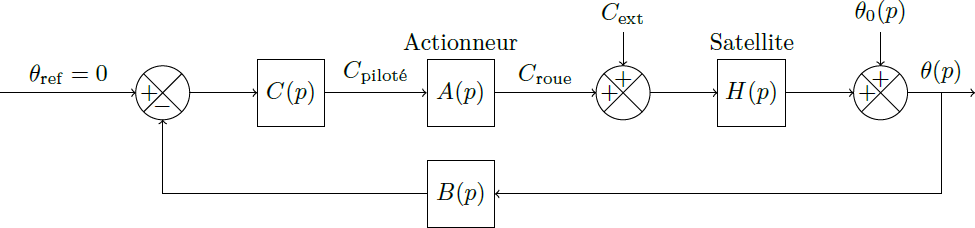
\includegraphics[width=\linewidth]{images/fig_12}
\caption{Schéma d’analyse pour la réponse aux conditions initiales \label{fig_12}}
\end{figure}
\fi

%\question{\label{q_24}}\textit{Déterminer $T_d(p)=\dfrac{C_{\text{piloté}}(p)}{\theta_0(p)}$ à partir des différentes fonctions de transfert de la \autoref{fig_12}. On note $c_{\text{pa}}(p)=c_{\text{piloté}}(t+\tau_1)$, avec $\tau_1 = \SI{0,7}{s}$. En déduire à partir de $T_d(p)$ l'expression de $\dfrac{C_{\text{pa}}}{\theta_0(p)}$.}% QUESTION ORIGINALE

\question{\label{q_24}\textit{En considérant que  $\theta_{\text{ref}}=0$ et  $C_{\text{ext}}=0$, déterminer $T_d(p)=\dfrac{C_{\text{piloté}}(p)}{\theta_0(p)}$ à partir des différentes fonctions de transfert de la \autoref{fig_12}. On note $c_{\text{pa}}(t)=c_{\text{piloté}}(t+\tau_1)$, avec $\tau_1 = \SI{0,7}{s}$. En déduire à partir de $T_d(p)$ l'expression de $\dfrac{C_{\text{pa}}(p)}{\theta_0(p)}$.}} % Question modifiée
\ifprof
\begin{corrige}
Dans les conditions énoncées : $C_{\text{piloté}}(p)=-\theta(p) B(p) C(p)$. De plus,$\theta(p)=\theta_0(p)+C_{\text{piloté}}(p) A(p) H(p)$. 
On a donc $C_{\text{piloté}}(p)=-\left( \theta_0(p)+C_{\text{piloté}}(p) A(p) H(p) \right) B(p) C(p)$.
En conséquences, $C_{\text{piloté}}(p)\left( 1+ A(p) H(p) B(p) C(p) \right)=- \theta_0(p) B(p) C(p)$.
Au final, $T_d(p)=\dfrac{C_{\text{piloté}}(p)}{\theta_0(p)} = -\dfrac{ B(p) C(p)}{ 1+ A(p) H(p) B(p) C(p)}$.


 On a $c_{\text{pa}}(t)=c_{\text{piloté}}(t+\tau_1)$ $\Leftrightarrow c_{\text{pa}}(t-\tau_1)=c_{\text{piloté}}(t) $ . En utilisant le théorème du retard, et en passant dans le domaine de Laplace, 
  $C_{\text{pa}}(p)e^{-\tau_1 p} =C_{\text{piloté}}(p)$. 
  
Or, $T_d(p)=\dfrac{C_{\text{piloté}}(p)}{\theta_0(p)}$; donc $T_d(p)=\dfrac{C_{\text{pa}}(p)e^{-\tau_1 p}}{\theta_0(p)}$.


\end{corrige}
\else
\fi

\question{\label{q_25}\textit{En utilisant le théorème de la valeur initiale,
ou toute autre méthode de votre choix, déterminer littéralement
et numériquement $c_{\text{pa}}(0)$ en réponse à une condition initiale 
$\theta_0(t)=\Theta_0 \gamma(t)$ d'amplitude $\Theta_0 = 20\degres$. En
déduire $c_{\text{piloté}}(\tau_1)$. 
[Remarques : $\gamma(t)$ désigne l’échelon d’Heaviside d’amplitude 1. On admettra que la valeur déterminée est proche de la 
valeur maximale (en valeur absolue) de celle obtenue pour des cas d’utilisation
de filtres $F(p)$ d'ordre supérieur à~1.]}}
\ifprof
\begin{corrige}

\begin{center}
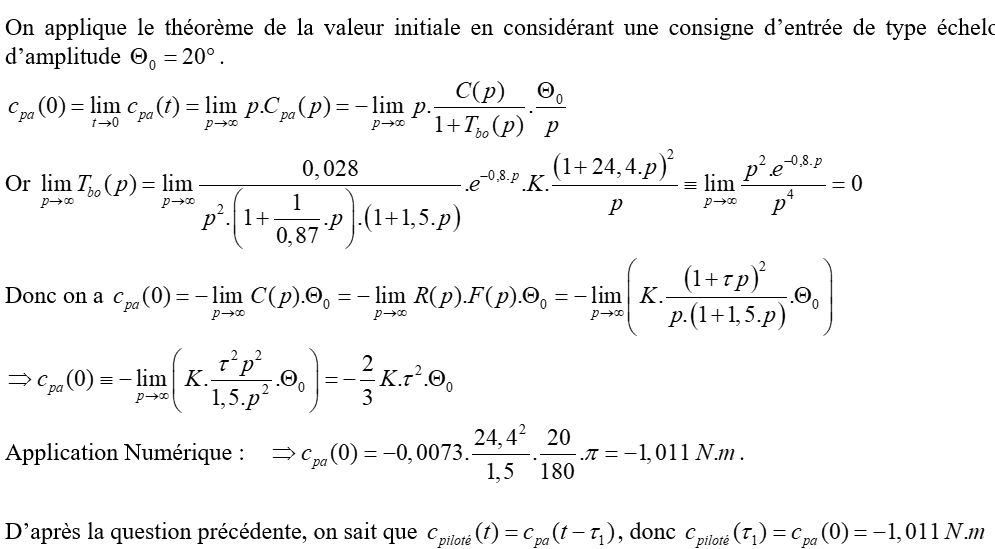
\includegraphics[width=\linewidth]{images/cor_q25}
\end{center}
%
%D'après la question précédente,  $C_{\text{pa}}(p) = T_d(p) \theta_0(p)  e^{\tau_1 p}$.
%
%Par application du théorème de la valeur initiale, 
%
%$c_{\text{pa}}(0) = \lim\limits_{p \to \infty} p T_d(p) \theta_0(p)  e^{\tau_1 p} $. Or $\theta_0(p) = \dfrac{\Theta_0}{p}$; donc 
%
%$c_{\text{pa}}(0) = \lim\limits_{p \to \infty}   -\dfrac{ B(p) C(p)}{ 1+ A(p) H(p) B(p) C(p)}  \Theta_0  e^{\tau_1 p}  $
%
%$c_{\text{pa}}(0) = \lim\limits_{p \to \infty}   -\dfrac{e^{-0,7p} C(p)}{ 1+ \dfrac{1}{1+\dfrac{1}{0,87}p}e^{-0,1 p}  \dfrac{0,028}{p^2} e^{-0,7p} C(p)}  \Theta_0  e^{\tau_1 p}  $
%
%$c_{\text{pa}}(0) = \lim\limits_{p \to \infty}   -\dfrac{e^{-0,7p}}{ 1+ \dfrac{1}{1+\dfrac{1}{0,87}p}e^{-0,1 p}  \dfrac{0,028}{p^2} e^{-0,7p} \dfrac{K(1+\tau p)^2}{p}}  \Theta_0  e^{0,7 p}   \dfrac{K(1+\tau p)^2}{p}$
%
%$c_{\text{pa}}(0) = \lim\limits_{p \to \infty}   -\dfrac{ 1+\dfrac{1}{0,87}p}{p^2+\dfrac{1}{0,87}p^3+  0,028 e^{-0,8p} K(1+\tau p)^2}   p^2\Theta_0  K(1+\tau p)^2  $
%
%
%A REVOIR !!
%
%$c_{\text{pa}}(0) = \lim\limits_{p \to \infty}   -\dfrac{ B(p) C(p)}{ 1+ A(p) H(p) B(p) C(p)}  \Theta_0  e^{-\tau_1 p}  $
%
%$c_{\text{pa}}(0) = \lim\limits_{p \to \infty}   -\dfrac{ 0 K\tau^2/1,5}{ 1+ 0\times 0 \times 0 K\tau^2/1,5}  \Theta_0  \times 0 $

\end{corrige}
\else
\fi

\question{\label{q_26}\textit{En réponse à une condition initiale  $\theta_0(t)=\Theta_0 \gamma(t)$ d’amplitude 20\degres, 
la \autoref{fig_13} montre l’évolution de la vitesse de rotation angulaire $\dot{\theta}$
autour de l’axe $\vect{y}$. À partir de la relation obtenue à la question \ref{q_10}, déterminer
la valeur maximale de la vitesse angulaire de la roue de réaction $\omega_r$.
Effectuer l’application numérique pour
$I_y = \SI{35,7}{kg.m^2}$ et $I_{\text{ry}}=\SI{4e-4}{kg.m^2}$.}}
\ifprof
\begin{corrige}
La question \ref{q_10} a permis d'établir que $I_y \dot{\theta}(t)=-I_{\text{ry}}\omega_r(t)$. D'après la figure, $| \dot{\theta}|_{\text{max}} \simeq \SI{3}{\degres.s^{-1}}$. 
On a donc $\omega_r(t) =  \dfrac{I_y}{I_{\text{ry}}} \dot{\theta}$ $=- \dfrac{35,7}{4\times 10^{-4}} \times 3 = \SI{267750}{\degres.s^{-1}} = \SI{44625}{tr.min^{-1}}$.
\end{corrige}
\else
\fi

\question{\label{q_27}\textit{Conclure alors sur la capacité de la loi de commande à satisfaire les contraintes imposées par l’actionneur
à roue de réaction.}}
\ifprof
\begin{corrige}
D'après le cahier des charges : 
\begin{itemize}
\item couple maximal : $\SI{0,005}{Nm} << \SI{1}{Nm}$;
\item vitesse maximale : $\SI{2800}{tr.min^{-1}} << \SI{44625}{tr.min^{-1}}$.
\end{itemize}

Les performances ne sont donc pas vérifiées.

\end{corrige}
\else
\fi

\subsubsection{\label{sec:3:D:2} Amélioration des performances vis-à-vis du dépointage initial}

\ifprof
\else

On note $\Delta \theta = \theta_{\text{ref}}-\theta$. La loi de commande déterminée précédemment est modifiée en ajoutant une nouvelle
fonction. Ainsi, avec la nouvelle architecture envisagée, la régulation se décompose en deux parties :
\begin{itemize}
\item pour un écart angulaire $|\Delta \theta|<0,3\degres$, la régulation se fait en position en utilisant le correcteur $C(p)$ déterminé
précédemment ;
\item pour un écart angulaire $|\Delta \theta|<0,3\degres$, le couple demandé à la roue de réaction est donné par $C_{\text{piloté}}(p)= -R_1(p)\left( b_v \text{sign}(\Delta \theta) + p\theta(p)\right))$ où $\text{sign}$ représente la fonction signe. L’objet de cette phase de l’étude est de
déterminer les paramètres de la nouvelle fonction. La synthèse de la fonction de transfert $R_1(p)$ et la gestion
de la commutation entre les deux parties de la loi de commande est hors du cadre de cette étude.
\end{itemize}
\fi


\question{\label{q_28}\textit{Justifier que pour $|\Delta \theta|> 0,3 \degres$, la deuxième composante de la loi de commande est une régulation de
vitesse avec une consigne de vitesse $\dot{\theta}_c(t)$ constante.}}
\ifprof
\begin{corrige}
\end{corrige}
\else
\fi

\question{\label{q_29}\textit{On admet que $I_y \dot{\theta}(t)=-I_{\text{ry}}\omega_r(t)$. Déterminer la valeur maximale
$|\dot{\theta}_c|_{\text{max}}$ (en \si{\degres.s^{-1}}) 
de la consigne de vitess $\dot{\theta}_c(t)$ que l’on peut imposer. Effectuer l’application numérique pour $I_y = \SI{35,7}{kg.m^2}$, $I_{\text{ry}}=\SI{4e-4}{kg.m^2}$ et une vitesse maximale de la roue de \SI{2800}{tr.min^{-1}} (correspondant à la vitesse maximale
de l’actionneur donnée par le tableau de la \autoref{fig_09}).}}
\ifprof
\begin{corrige}
La question \ref{q_10} a permis d'établir que $I_y \dot{\theta}(t)=-I_{\text{ry}}\omega_r(t)$.

On a donc $\left| \omega_r(t) \right| = \dfrac{I_{\text{ry}}}{I_y}\left|\dot{\theta}(t)\right|$ 
$=\dfrac{4\times 10^{-4}}{35,7} \times 2800 =\SI{0,03}{tr.min^{-1}}=\SI{0,19}{\degres.s^{-1}} $.
\end{corrige}
\else
\fi

\ifprof
\else

\begin{figure}[H]
\centering
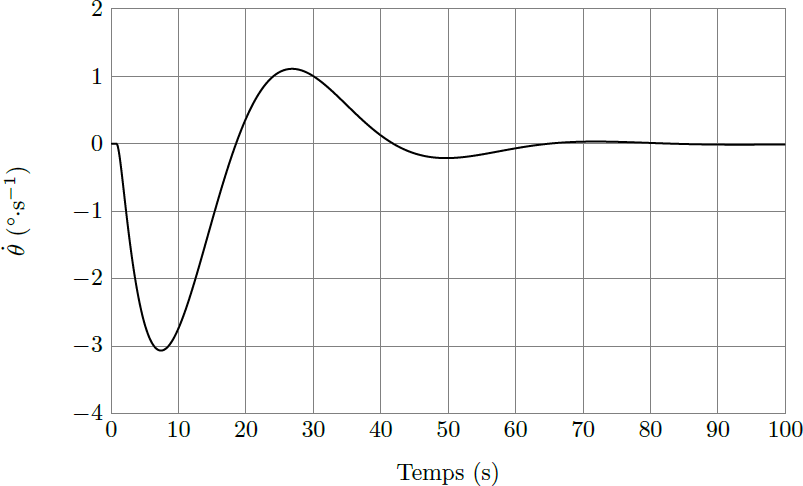
\includegraphics[width=.7\linewidth]{images/fig_13}
\caption{Évolution de la vitesse de rotation du satellite $\dot{\theta}$ (\si{\degres.s^{-1}}) en réponse à un dépointage initial de 20\degres \label{fig_13}}
\end{figure}
\fi


\question{\label{q_30}\textit{La \autoref{fig_14} montre les réponses obtenues (en utilisant un simulateur trois axes comportant en particulier les modes oscillants dus aux souplesses de la structure) avec la loi de commande définie précédemment pour un dépointage initial $\Theta_0 = 20\degres$. Commenter les réponses obtenues et conclure alors sur la capacité de la nouvelle loi de commande à satisfaire l’ensemble des contraintes imposées par le cahier des charges.}}
\ifprof
\begin{corrige}
D'après le cahier des charges : 
\begin{itemize}
\item couple maximal : $\SI{0,005}{Nm}$ : l'exigence est respectée, sauf ponctuellement au démarrage de la roue à réaction et au changement de loi de commande à $t=\SI{1300}{s}$;
\item vitesse maximale : $\SI{2800}{tr.min^{-1}} = \SI{293}{rad.s^{-1}}$ : l'exigence est respectée, car la vitesse reste inférieure à $\SI{35}{rad.s^{-1}}$.
\end{itemize}
Ces résultats permettent de valider la nouvelle loi de commande.
\end{corrige}
\else
\fi

\ifprof
\else

\begin{figure}[H]
\centering
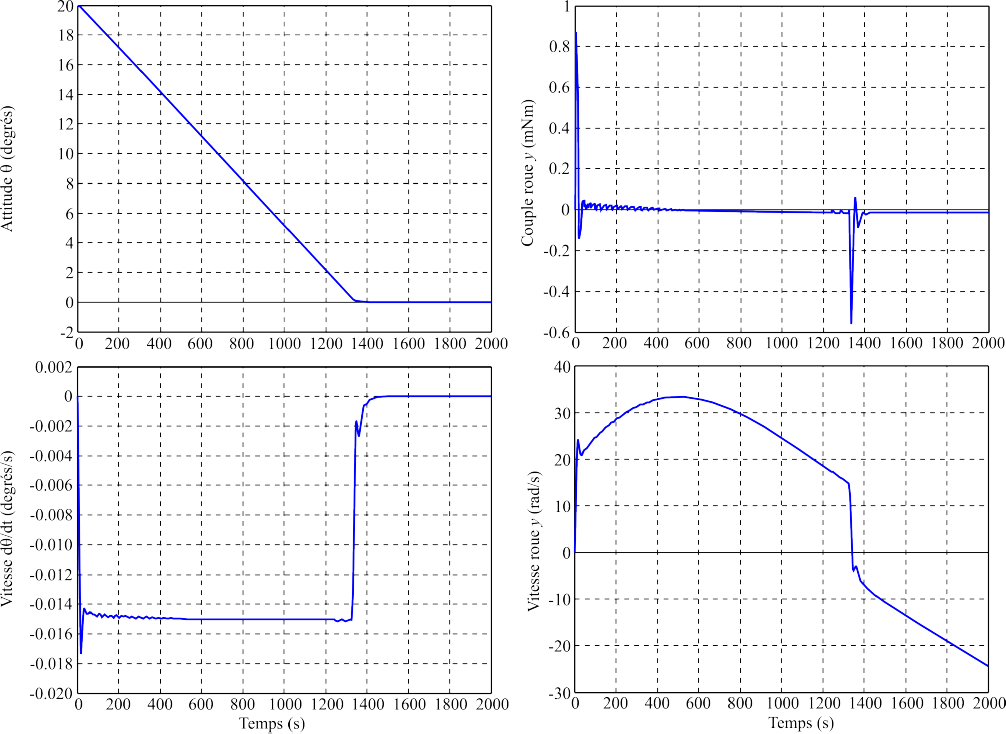
\includegraphics[width=.8\linewidth]{images/fig_14}
\caption{Évolutions temporelles à partir d’une condition initiale (dépointage) $\theta_0 = 20\degres$ \label{fig_14}}
\end{figure}
\fi

\subsubsection{\label{sec:3:D:3} Analyse des performances vis-à-vis d’un couple perturbateur constant}

L’objet de cette partie est d’analyser les performances de la loi de commande lorsque le satellite est soumis à
un couple extérieur constant, $C_{\text{ext}}= C_0 \gamma(t)$ d’amplitude $C_0 =\SI{e-6}{Nm}$.

\question{\label{q_31}\textit{Sans calcul, mais en justifiant votre réponse, préciser l’écart en régime permanent en réponse à un couple
perturbateur constant.}}
\ifprof
\begin{corrige}
$C(p)=K\dfrac{\left(1+\tau p\right)^2}{p}$. Le correcteur contient une action intégrale en amont de la perturbation. Pour une perturbation constante, l'écart en régime permanent est donc nul.
\end{corrige}
\else
\fi
%
%\question{\label{q_32}}\textit{À partir du schéma de la \autoref{fig_11}, déterminer la valeur du couple appliqué $C_{\text{roue}}$ en régime permanent
%en réponse au couple perturbateur $C_{\text{ext}}(t)$ supposé constant et en déduire la loi temporelle d’évolution de la
%vitesse de la roue. Quelle est la conséquence sur le fonctionnement de l’actionneur du couple perturbateur ? Justifier le terme de «~saturation~» pour décrire ce phénomène. À partir de quel horizon temporel survient cette
%situation ?}
%\ifprof
%\begin{corrige}
%On a $C_{\text{ext}}(t) = C_0 =\SI{e-6}{Nm}$. En régime permanent, $C_{\text{roue}}$ doit être égal à $-C_0 =-\SI{e-6}{Nm}$.
%
%Par application du théorème du moment dynamique appliqué à la roue à réaction : $C_{\text{ext}}(t) = I_{ry} \dot{\omega}_r(t)$. On a donc $\omega_r(t) = -\dfrac{C_0}{I_{ry}}t + \text{cte}$.
%
%Pour maintenir le couple désiré, il faut dont que la vitesse tende vers l'infini. La vitesse saturera donc à partir d'un certain seuil (ici \SI{2800}{tr/min}). 
%
%En prenant la constante nulle, on a  $|\omega_r(T)| = \dfrac{C_0}{I_{ry}}T$ soit $T = \dfrac{2800 \times 2\pi}{60} \times 10^{6} \times 4\times 10 ^{-4} $ $=\SI{117 286}{s} \simeq \SI{32,5}{h}$.
%
%
%\end{corrige}
%\else
%\fi
%
%\ifprof
%\else
%
%
%Pour remédier au problème de saturation, on utilise des bobines magnétiques, appelées magnétocoupleurs, qui
%permettent de créer des moments adaptés grâce à l’action du champ magnétique terrestre. Le satellite est équipé
%de trois magnétocoupleurs orientés respectivement selon les trois directions $\vect{x}$, $\vect{y}$ et $\vect{z}$ du satellite, et dont on peut
%commander précisément les moments magnétiques respectifs $\vect{\mathcal{M}}_x=\mathcal{M}_x\vect{x}$, $\vect{\mathcal{M}}_y=\mathcal{M}_y\vect{y}$ et $\vect{\mathcal{M}}_z=\mathcal{M}_z\vect{z}$. Dans
%le cas d’une orbite polaire, le champ magnétique terrestre a pour expression $\vect{B}=B_0 \cos\left(\omega_0 t\right) \vect{x} +2 B_0 \sin\left(\omega_0 t\right) \vect{z}.$ L’interaction entre les magnétocoupleurs et le champ magnétique terrestre se traduit par un moment (mécanique)
%dont l’expression au centre d’inertie $G$ du satellite est :
%$$
%\vect{M}_G (\text{magnétique}) = 
%B_0 \left( 
%2\mathcal{M}_y \sin \left(\omega_0 t \right) \vect{x}
%+ \left(
%\mathcal{M}_z \cos \left(\omega_0 t \right) 
%-2\mathcal{M}_x \sin\left(\omega_0 t \right) \right)\vect{y}
%-\mathcal{M}_y \cos \left(\omega_0 t \right) \vect{z}
%\right).
%$$
%\fi
%
%\question{\label{q_33}}\textit{Expliquer comment les magnétocoupleurs peuvent permettre de résoudre le problème de saturation des
%roues de réaction : on détaillera précisément quel est le rôle de chacun des trois magnétocoupleurs et à quels
%instants de l’orbite du satellite leurs effets sont les plus sensibles.}
%\ifprof
%\begin{corrige}
%Les magnétocoupleurs coupleurs permettent d'apporter un couple supplémentaire pour remédier au problème de saturation.... 
%\end{corrige}
%\else
%\fi